% !TeX spellcheck = ru_RU-Russian

\documentclass{beamer}
\mode<presentation>
\usetheme{Ilmenau}

\usepackage[utf8]{inputenc}
\usepackage[T1,T2A]{fontenc}
\usepackage{tikz}

\def \MinSize {22}

\tikzstyle{fcnode}=[
  thick,
  draw=black,
  rectangle,
  minimum height=2*\MinSize,
  minimum width=1.5*\MinSize
]

\tikzstyle{neuron}=[
  thick,
  draw=black,
  circle,
  minimum size=\MinSize
]

\begin{document}

\section{Модель нейрона}

\begin{frame}
  \begin{columns}

    \begin{column}{0.5\textwidth}
      $$ y = \sum_{i}^{} w_i \cdot x_i + b $$
    \end{column}

    \begin{column}{0.5\textwidth}
      \begin{center}
        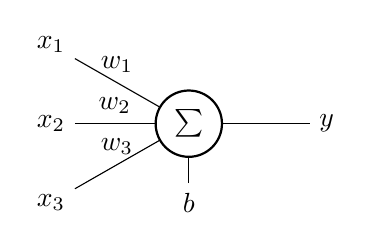
\begin{tikzpicture}
          \def \x {3}
          \def \y {0}
          \def \xOff {1.75}
          \def \yOff {1}

          \node[neuron] (n1) at (\x, \y) {$\sum$};

          % ins
          \node (x1) at (\x - \xOff, \y + \yOff) {$x_1$};
          \node (x2) at (\x - \xOff, \y) {$x_2$};
          \node (x3) at (\x - \xOff, \y - \yOff) {$x_3$};
          \node (b1) at (\x, \y - \yOff) {$b$};

          % out
          \node (y1) at (\x + \xOff, \y) {$y$};

          % connect ins
          \foreach \i in {1,...,3}{
            \draw (x\i) -- (n1) node[midway,above] {$w_\i$};
          }
          \draw (b1) -- (n1);

          % connect out
          \draw (n1) -- (y1);
        \end{tikzpicture}
      \end{center}
    \end{column}

  \end{columns}
\end{frame}

\begin{frame}

\end{frame}

\section{Введение}

\section{Перцептрон}

\section{Функция активации}

\end{document}
